\section{结果分析与检验}
\label{sec:results}

\subsection{已完成结果的汇总}
问题一的三项结果已在第~\ref{sec:q1}~节随模型给出，此处汇总其检验状态。

验证清单按结论逐项记录如下：质量评分方案通过六方案秩相关与名次变化检验（图~\ref{fig:q1-nature-06}）；
扩展集域内质量稳定性通过 arxiv/github 新增前后域均分对照检验（表~\ref{tab:q1-domain-score}，仅两域有扩展数据）；
语料级下降由构成变化解释通过顺序恒等分解检验（图~\ref{fig:q1-nature-04}）；冲突率在扩展集的一致性通过分层覆盖率
与重加权对照检验（表~\ref{tab:q1-conflict-coverage}，两域）；冲突判定的阈值敏感性通过三组分位数敏感性检验（图~\ref{fig:q1-conflict-02}，结论为条件性）；
有限补偿单调性与闭式解已完成代数核验与合成接口测试。评分与真实质量的一致性、冲突误判率与因果机制、bootstrap 区间与权重扰动仍待 A18 原始文本抽检、83 条分层清单人工标注和重抽样检验；配比模型跨尺度绝对预测已由重复设计配对下界分析证实不可辨识，属于排除性结论。

\subsection{检验策略说明}
本文区分三类检验。\emph{内部一致性检验}（复算误差、类别穷尽性、单调性）保证实现与公式一致；\emph{敏感性检验}（六评分方案、三阈值组、五维权重扰动）保证结论不依赖单一建模选择；\emph{外部效度检验}（A18 原始文本抽检、人工标注清单、下游损失关联）锚定评分与真实质量的关系，其中后一类在本版本中部分待完成，已在上述清单中如实标注，不作为已成立结论使用。

\subsection{已知局限}
其一，外部效度锚定尚不完整，质量分数的绝对水平解释需谨慎；其二，冲突消解的阈值与五维分组是两个主要自由度，本文冻结处理并报告敏感性，未做全组合稳健性扫描；其三，配比模型的跨尺度结论局限于相对排序，绝对损失外推已被排除但未解决；其四，问题三子问题二、三虽已接入条件结果，问题二至问题四的其余正式章节仍待定稿。

\section{问题三的条件资源配置结果}
\label{sec:q3-results}

问题三的正文按“问题分析—模型与求解—情景结果—数值复核—结果边界”的层级组织。
本节按子问题顺序接入 M0 的 $N$--$D$ 基线、M1 原生 $Q_B$ 条件优化，以及
M2/P 配比条件面板和 Q2--Q3 假设接口；三类结果保持数据来源、量尺和证据状态的区分。

% 问题三 6.1--6.3：问题分析、数据预分析与目标函数。
% 依据 q3-conditional-resource.tex 及其 outline 整理为仓库正文片段。
% 本文件不定义文档环境，不单独编译。

\subsection{问题分析}
\label{sec:q3-analysis}

\subsubsection{问题要求与求解对象}

问题三要求在给定计算预算和上下文条件下配置模型规模、训练数据量及质量资源，
使预测损失尽可能小。前两问提供的数据没有统一的样本级连接键，因此不能把
$N$、$D$、$Q_B$、$p$ 和 $Q_A(p)$ 直接拼接为一个已验证的联合样本表。其中，
$N$ 和 $D$ 来自 B1，$Q_B$ 是 B6/B7 的原生质量分数，$p$ 和 $Q_A(p)$ 来自
A4/A5 的配比面板。本文据此将问题三定义为条件资源配置问题。

求解对象分为三层递进分析：第一层使用 B1 的 $N$--$D$ 数据建立 M0 基线；
第二层使用 B6/B7 的原生 $Q_B$ 建立 M1 的 $N$--$D$--$Q_B$ 条件优化；
第三层以 A4/A5 中实际观测的配比候选生成情景，通过显式标注的假设接口构造
对应的 $Q_B$，再调用 M1 求解器得到资源配置面板。三层结果不混合拟合。

本节所称“最优”均限定为给定模型、预算、上下文、质量成本、支持域和接口映射下的
情景内最优。由于 A、B 数据缺少共同连接键，且接口标度和成本函数仍是条件假设，
当前结果不能识别现实中的唯一最优配比，也不能识别支持域外的全局最优。

\subsubsection{问题三与前两问的衔接}

问题二的 B1 数据提供规模基线，B6/B7 数据提供含原生质量变量的条件模型，问题一
提供有限个已观测配比候选及其 A 侧质量标签。由于 A、B 数据缺少共同连接键，且
$Q_A$ 与 $Q_B$ 尚未统一标度，本文不把四量模型写成已验证的联合实证模型，也不
把 $Q_A$ 直接代入 B 侧 Loss。

\subsubsection{求解路线}

本文按“冻结数据与版本—建立 M0、M1、M2/P 三层条件模型—施加预算、支持域、
上下文和质量成本约束—解析解与多起点 SLSQP 求解—有限性、哈希、预算误差、
参数折叠和边界检查—输出条件情景”的路线组织结果。该路线保留了探索性计算、
条件结论和不可识别接口之间的边界。

\subsection{数据预分析与变量说明}
\label{sec:q3-data}

\subsubsection{数据角色和规模}

问题三使用的数据角色、规模和用途按条目说明如下：B1 有 1,176 行，用于 M0 参数估计和
$N,D$ 支持域确定；B6 有 360 行，用于 M1 原生 $Q_B$ 条件模型；B7 是 B6 的嵌套扩展，
仅用于条件核验，不重复计权；C7 提供 5 个上下文值，用于 $L_{\rm ctx}$ 场景；A4/A5
提供 6 个观测配比候选，用于 M2/P 离散配比情景。

\subsubsection{变量、量纲与支持域}

$N$ 表示模型参数规模（十亿参数），$D$ 表示训练数据规模（十亿 tokens），
$L_{\rm ctx}$ 表示上下文长度，$Q_B$ 表示 B6/B7 原生质量分数。配比向量
$p=(p_1,\ldots,p_J)$ 满足
\begin{equation}
 Q_A(p)=q^\top p=\sum_{j=1}^{J}q_jp_j,
 \qquad p_j\ge0,\qquad \sum_{j=1}^{J}p_j=1.
 \label{eq:q3-overview-qa}
\end{equation}
$Q_A(p)$ 保留在 Q1 的 $0$--$100$ 候选尺度，$Q_B$ 使用 B6/B7 的
$0.1$--$1.0$ 原生尺度，二者不直接相等。

M0 和 M1 的资源配置均限制在 B1 的观测支持域
\begin{equation}
 N\in[0.070542,11.965825],\qquad
 D\in[0.134,299.893],
 \label{eq:q3-overview-support}
\end{equation}
M1 额外满足
\begin{equation}
 Q_B\in[0.1,1.0],\qquad Q_0=0.1.
 \label{eq:q3-overview-q-domain}
\end{equation}

\subsubsection{数据排除和版本边界}

B8 不进入问题三主拟合；C8 中的 4 个截断 JSON 不进入当前 Q3 主输入；
M0/M1 参数折叠只用于不确定性传播，不重新拟合模型；A--B 行级连接、正式
M3 联合拟合和未经验证的质量桥接均保持关闭。所有支持域外点和边界点在输出中
单独标记。

\subsection{目标函数、预算约束与求解方法}
\label{sec:q3-objective}

\subsubsection{规模损失函数}

M0 的 B1 条件损失为
\begin{equation}
 \widehat L_{\mathrm{M0}}(N,D)=E+A N^{-\alpha}+B D^{-\beta}.
 \label{eq:q3-overview-m0}
\end{equation}
M1 在 B6/B7 原生质量变量下为
\begin{equation}
 \widehat L_{\mathrm{M1}}(N,D,Q_B)
 =E+A N^{-\alpha}+B D^{-\beta}+G(1-Q_B).
 \label{eq:q3-overview-m1}
\end{equation}
M1 的 $Q_B$ 只表示 B6/B7 原生质量变量，不替代 Q1 的 $Q_A$。

\subsubsection{成本函数与预算约束}

基础规模成本采用上下文修正的乘积形式
\begin{equation}
 C_{\mathrm{base}}=10^{18}ND(6+\eta L_{\rm ctx}),
 \qquad \eta=2\times10^{-4},
 \label{eq:q3-overview-base-cost}
\end{equation}
质量增量成本为
\begin{equation}
 C_Q=10^9D\,[g(Q_B)-g(Q_0)].
 \label{eq:q3-overview-quality-cost}
\end{equation}
本文将指数、幂函数和对数渐进三类 $g$ 分开比较，不把它们混合为一个确定的
真实成本律。预算集合为
\begin{equation}
 C_{\mathrm{base}}+C_Q\le C,qquad
 C\in\{10^{19},10^{22},10^{24}\},qquad
 L_{\rm ctx}\in\{2048,4096,8192,32768,131072\}.
 \label{eq:q3-overview-constraints}
\end{equation}

\subsubsection{约束集合与数值方法}

统一约束还包括式~\eqref{eq:q3-overview-support} 的 $N,D$ 支持域和式
~\eqref{eq:q3-overview-q-domain} 的 $Q_B$ 支持域。M0 先利用平滑预算约束
推导解析候选，再用有界多起点 SLSQP 复核；M1 对正值变量采用对数参数化，
从多个确定性起点执行 SLSQP；M2/P 固定接口产生的假设 $Q_B$，复用冻结的 M1
求解器。当前模型维度低、目标函数光滑、约束明确，故不采用遗传算法或粒子群
算法。每个情景均检查预算可行性、有限性、收敛状态、边界状态和支持域角色。

% 问题三·子问题一：M0 的 N-D 基线优化
% 本文件为正文片段，遵循 paper/main.tex 的唯一入口约定；不定义文档环境。
% 证据运行：q3-nd-baseline-20260925-r01。

\subsection{问题三子问题一：M0 的 $N$--$D$ 基线优化}
\label{sec:q3-m0-nd}

问题三子问题一研究给定算力预算和上下文长度下参数规模 $N$ 与训练数据规模
$D$ 的资源分配。为保持问题二中不同数据角色的边界，本节固定
$Q=Q_0$、$p=p_0$，采用 B1/Pythia 条件下的 $N$--$D$ 标度律，
不能直接解释为跨来源的联合最优配置。

本节使用问题二 M0 的 B1/Pythia 拟合参数
\[
E=1.689798,\qquad
A=0.353980,\qquad
B=1.240306,\qquad
\alpha=0.339977,\qquad
\beta=0.279878 .
\]
其中 $N$ 以十亿参数（B）计，$D$ 以十亿 token（B）计。B1 的观测支持域为
\[
N\in[0.070542,11.965825],\qquad
D\in[0.134,299.893].
\]

\subsubsection{解析解}
\label{sec:q3-m0-nd-analytic}

在 $Q$ 和 $p$ 固定时，M0 的预测损失函数为
\begin{equation}
\widehat L(N,D)=E+A N^{-\alpha}+B D^{-\beta}.
\label{eq:q3-m0-loss}
\end{equation}

上下文长度 $L_{\rm ctx}$ 由 C7 架构元数据外生给定，考虑长文本注意力开销后，预算约束按十亿单位换算为
\begin{equation}
10^{18}\bigl(6+\eta L_{\rm ctx}\bigr)ND\le C,
\qquad \eta=2\times10^{-4}.
\label{eq:q3-m0-budget}
\end{equation}
记预算允许的规模乘积为
\begin{equation}
K(C,L_{\rm ctx})
=\frac{C}{10^{18}\bigl(6+\eta L_{\rm ctx}\bigr)}.
\label{eq:q3-m0-k}
\end{equation}

由于 $A,B,\alpha,\beta>0$，有
\begin{equation}
\frac{\partial \widehat L}{\partial N}
=-\alpha A N^{-\alpha-1}<0,\qquad
\frac{\partial \widehat L}{\partial D}
=-\beta B D^{-\beta-1}<0.
\label{eq:q3-m0-first-derivative}
\end{equation}
在不考虑支持域上界时，最优点会用尽预算，即 $ND=K$。将等式约束代入
拉格朗日一阶条件，得到
\begin{equation}
\alpha A N^{-\alpha}=\beta B D^{-\beta},
\qquad ND=K .
\label{eq:q3-m0-balance}
\end{equation}
由此得到预算约束下的无界解析解
\begin{equation}
N_{\rm rel}^{*}
=\left(\frac{\alpha A}{\beta B}K^{\beta}\right)^{1/(\alpha+\beta)},
\qquad
D_{\rm rel}^{*}=\frac{K}{N_{\rm rel}^{*}} .
\label{eq:q3-m0-analytic-solution}
\end{equation}

式~\eqref{eq:q3-m0-balance} 表明，最优分配并不是令 $N$ 和 $D$ 的原始
边际收益相等，而是令两项的弹性加权贡献相等。边际收益递减可由二阶导数
直接验证：
\begin{equation}
\frac{\partial^2\widehat L}{\partial N^2}
=\alpha(\alpha+1)A N^{-\alpha-2}>0,\qquad
\frac{\partial^2\widehat L}{\partial D^2}
=\beta(\beta+1)B D^{-\beta-2}>0 .
\label{eq:q3-m0-diminishing-return}
\end{equation}
因此，增加 $N$ 或 $D$ 均能降低 Loss，但单位资源带来的下降幅度会随相应
资源规模增大而减小。解析解只有在
$(N_{\rm rel}^{*},D_{\rm rel}^{*})$ 落在 B1 支持域内时，才可被解释为
支持域内候选。

C7 中观测到的上下文长度为
\[
L_{\rm ctx}\in\{2048,4096,8192,32768,131072\}.
\]
注意力项系数与基础训练项系数相等的临界上下文长度为
\begin{equation}
L_{\rm ctx}^{\rm crit}=\frac{6}{\eta}=30000.
\label{eq:q3-m0-critical-context}
\end{equation}
该临界值位于 $8192$ 和 $32768$ 之间，因此这两个相邻的 C7 取值可以
用于观察注意力开销跨过临界水平时的资源收缩现象。

\subsubsection{有界数值求解}
\label{sec:q3-m0-nd-bounded}

解析解没有考虑 B1 的观测支持边界。为避免把超出观测范围的点误写成已验证
配置，进一步求解
\begin{equation}
\begin{aligned}
\min_{N,D}\quad &\widehat L(N,D)\\
\mathrm{s.t.}\quad
&ND\le K(C,L_{\rm ctx}),\\
&0.070542\le N\le11.965825,\\
&0.134\le D\le299.893 .
\end{aligned}
\label{eq:q3-m0-bounded-problem}
\end{equation}

数值求解在 $(\log N,\log D)$ 空间中进行，以保持正值并改善不同量级下的
数值条件。每个预算--上下文情景使用六个确定性起点：无界解析解、四个
支持域角点和对数尺度中心点；随后采用带显式预算不等式的 SLSQP 求解。
候选解只有在预算残差满足
\begin{equation}
C-10^{18}\bigl(6+\eta L_{\rm ctx}\bigr)ND
\ge -\max\{1,10^{-10}C\}
\label{eq:q3-m0-feasibility}
\end{equation}
时才保留，并在保留的可行解中选择预测 Loss 最小者。该过程同时检查
预算可行性、$N,D$ 边界可行性和多起点结果的一致性。

15 个场景均得到有限的可行解。每个场景均保留六个起点，成功标记数为
5 或 6，个别场景出现两个数值上不同的情况，按预测 Loss 值选出的
结果与解析解在支持域内部一致到表中展示精度。

\subsubsection{结果分析}
\label{sec:q3-m0-nd-results}

表~\ref{tab:q3-m0-nd-scenarios} 汇总 15 个预算--上下文情景。
$N_{\rm rel}^{*},D_{\rm rel}^{*}$ 表示不加支持域边界的解析解，$N^{*},D^{*}$
表示有界 SLSQP 解。“$D_{\max}$”和“$N_{\max},D_{\max}$”表示有界解
触及相应 B1 支持上界；“域内”和“外推”针对无界解析解判定。

\begin{table}[htbp]
  \centering
  \caption{M0 在 15 个预算--上下文情景下的解析解与有界解}
  \label{tab:q3-m0-nd-scenarios}
  \scriptsize
  \setlength{\tabcolsep}{3pt}
  \renewcommand{\arraystretch}{1.12}
  \resizebox{\textwidth}{!}{%
  \begin{tabular}{rrrrrrrrll}
    \toprule
    $C$ (FLOPs) & $L_{\rm ctx}$ & $N_{\rm rel}^{*}$ & $D_{\rm rel}^{*}$
      & 解析 Loss & $N^{*}$ & $D^{*}$ & 有界 Loss
      & 边界 &求解范围\\
    \midrule
    $10^{19}$ & 2,048   & 0.2213 & 7.0497    & 2.9989 & 0.2213 & 7.0497   & 2.9989 & -- & 域内\\
    $10^{19}$ & 4,096   & 0.2152 & 6.8142    & 3.0114 & 0.2152 & 6.8142   & 3.0114 & -- & 域内\\
    $10^{19}$ & 8,192   & 0.2045 & 6.4031    & 3.0347 & 0.2045 & 6.4031   & 3.0347 & -- & 域内\\
    $10^{19}$ & 32,768  & 0.1634 & 4.8758    & 3.1412 & 0.1634 & 4.8758   & 3.1412 & -- & 域内\\
    $10^{19}$ & 131,072 & 0.1068 & 2.9078    & 3.3672 & 0.1068 & 2.9078   & 3.3672 & -- & 域内\\
    \midrule
    $10^{22}$ & 2,048   & 5.0069  & 311.6048  & 2.1432 & 5.2024 & 299.8930 & 2.1432 & $D_{\max}$ & 外推\\
    $10^{22}$ & 4,096   & 4.8688  & 301.1956  & 2.1475 & 4.8899 & 299.8930 & 2.1475 & $D_{\max}$ & 外推\\
    $10^{22}$ & 8,192   & 4.6256  & 283.0256  & 2.1556 & 4.6256 & 283.0256 & 2.1556 & -- & 域内\\
    $10^{22}$ & 32,768  & 3.6961  & 215.5177  & 2.1925 & 3.6961 & 215.5177 & 2.1925 & -- & 域内\\
    $10^{22}$ & 131,072 & 2.4152  & 128.5289  & 2.2707 & 2.4152 & 128.5290 & 2.2707 & -- & 域内\\
    \midrule
    $10^{24}$ & 2,048   & 40.0506 & 3,895.4695 & 1.9134 & 11.9658 & 299.8930 & 2.0934 & $N_{\max},D_{\max}$ & 外推\\
    $10^{24}$ & 4,096   & 38.9459 & 3,765.3416 & 1.9155 & 11.9658 & 299.8930 & 2.0934 & $N_{\max},D_{\max}$ & 外推\\
    $10^{24}$ & 8,192   & 37.0012 & 3,538.1924 & 1.9195 & 11.9658 & 299.8930 & 2.0934 & $N_{\max},D_{\max}$ & 外推\\
    $10^{24}$ & 32,768  & 29.5660 & 2,694.2546 & 1.9377 & 11.9658 & 299.8930 & 2.0934 & $N_{\max},D_{\max}$ & 外推\\
    $10^{24}$ & 131,072 & 19.3194 & 1,606.7809 & 1.9763 & 11.9658 & 299.8930 & 2.0934 & $N_{\max},D_{\max}$ & 外推\\
    \bottomrule
  \end{tabular}}
\end{table}

低预算 $10^{19}$ FLOPs 下，5 个上下文情景的解析解全部位于 B1 支持域内，
因此解析解与有界解重合。随着上下文从 2,048 增加到 131,072，$N^{*}$
从 0.2213 B 降至 0.1068 B，$D^{*}$ 从 7.0497 B tokens 降至 2.9078 B
tokens，Loss 从 2.9989 上升至 3.3672。这一变化来源于有效规模乘积 $K$
的减少。

中预算 $10^{22}$ FLOPs 下，$L_{\rm ctx}=2,048$ 和 $4,096$ 的无界解析解
分别给出 $D=311.6048$ B 和 $D=301.1956$ B，超过 B1 的
$D_{\max}=299.893$ B；有界求解把 $D$ 截在上界，并相应调整 $N$。
当上下文为 $8,192$ 或更大时，解析解重新回到 B1 支持域内部。因此，
该预算档同时展示了“支持域边界触及”和“上下文开销收缩后回到域内”两种情况。

高预算 $10^{24}$ FLOPs 下，5 个上下文情景的无界解析解都超出 B1 支持域，
且同时超过 $N_{\max}$ 与 $D_{\max}$。有界解在全部情景中均取
$N^{*}=11.965825$ B、$D^{*}=299.893$ B tokens，预测 Loss 均为 2.0934。
由于支持域上界已经限制了可用规模，实际消耗的算力仅约为
$2.30\times10^{22}$ 至 $1.16\times10^{23}$ FLOPs；未使用的预算不能
被解释为模型还可以在 B1 证据范围内继续获得的收益。高预算下无界解析
Loss（1.9134--1.9763）只能作为外推诊断，不能作为已验证的最优 Loss。


图~\ref{fig:q3-m0-nd-baseline}将表中的解析解、有界解和 B1 支持边界放在同一
$N$--$D$ 平面中。低预算点位于观测支持域内部，解析点与有界点基本重合；预算
升高后，解析前沿继续向支持域外延伸，而有界解在 $N_{\max}$ 或 $D_{\max}$
处停止。因而图中的边界点表达的是“在当前支持域内可取的最大配置”，不是对
支持域外模型规模的经验验证。

\begin{figure}[htbp]
  \centering
  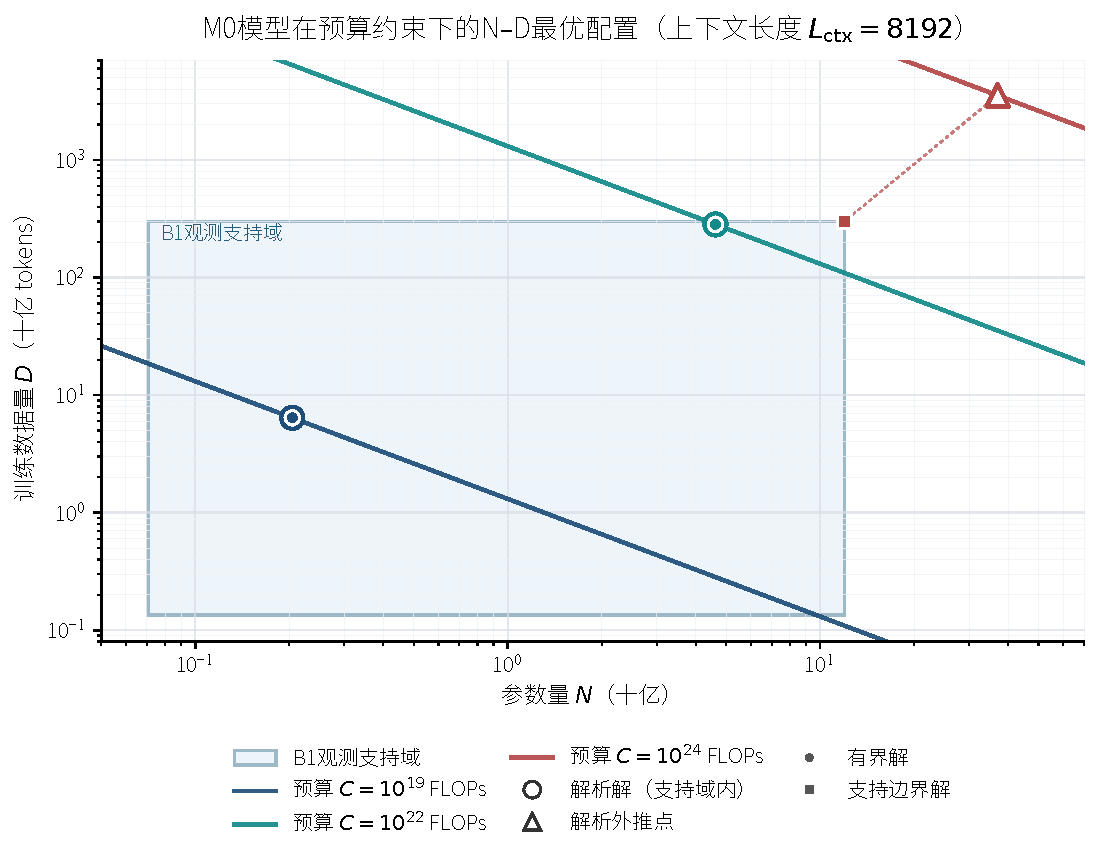
\includegraphics[width=0.82\textwidth]{figures/q3-nd-baseline-cn-v1/fig_q3_m0_nd_cn_single_v1.pdf}
  \caption{M0 在 $L_{\rm ctx}=8192$ 下的 $N$--$D$ 条件配置。空心点表示无界解析解，实心点表示 B1 支持域内的有界解，方形表示支持上界活跃的情景。}
  \label{fig:q3-m0-nd-baseline}
\end{figure}

图~\ref{fig:q3-m0-nd-budget}进一步将五档上下文和三档预算放在同一条件面板中。
随着 $L_{\rm ctx}$ 增加，注意力项压缩有效预算乘积，配置点沿着较低的 $N$--$D$
乘积移动；在 $10^{24}$ FLOPs 档，五个上下文均触及 B1 的双上界。这个图形只
是 15 个场景的可视化索引，数值判定仍以表~\ref{tab:q3-m0-nd-scenarios} 和
支持域约束为准。

\begin{figure}[htbp]
  \centering
  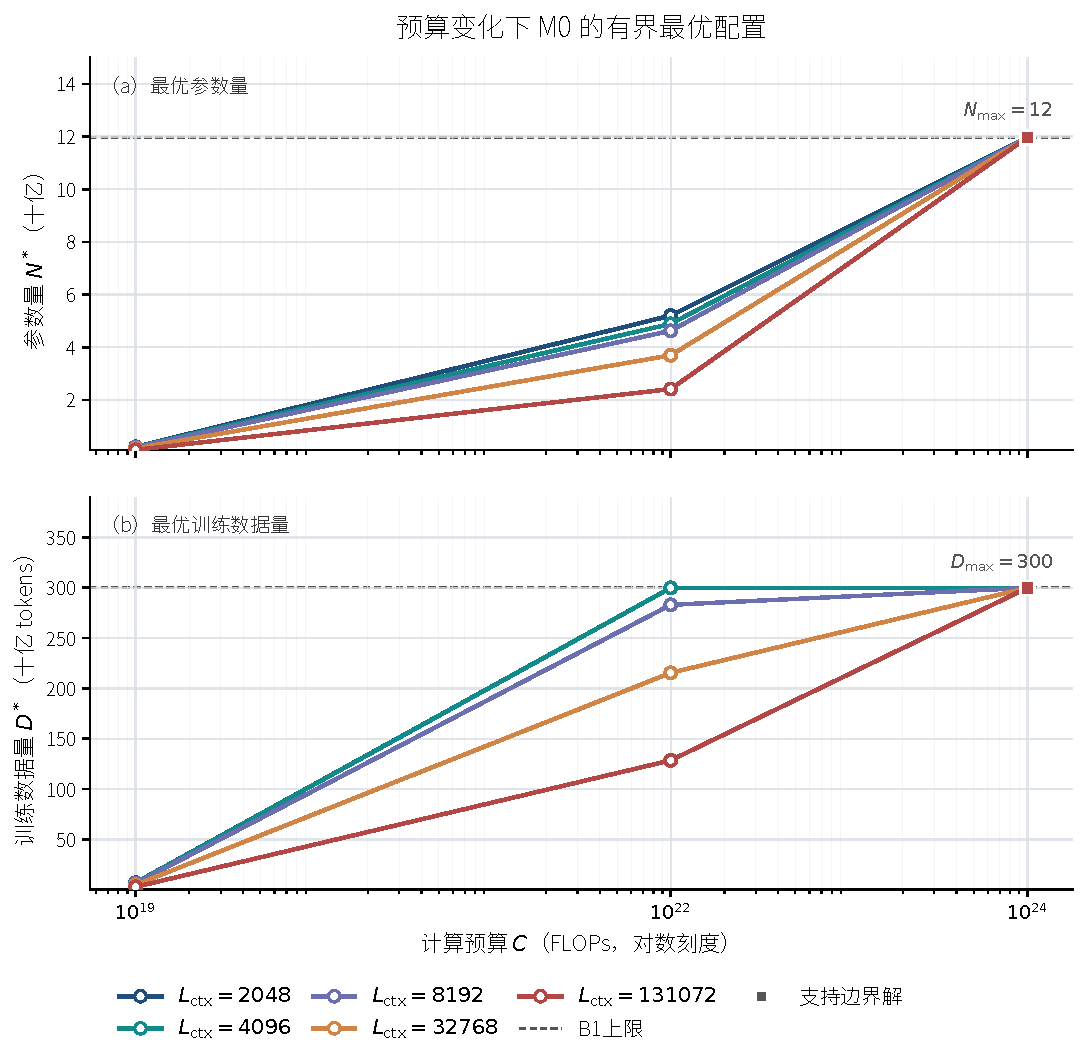
\includegraphics[width=0.78\textwidth]{figures/q3-nd-budget-cn-v1/fig_q3_m0_nd_budget_cn_single_v1.pdf}
  \caption{M0 在三档预算和五档上下文下的有界 $N$--$D$ 配置。虚线表示 B1 观测支持上限，方形表示边界约束活跃的场景。}
  \label{fig:q3-m0-nd-budget}
\end{figure}

\subsubsection{小结}

在 B1/Pythia 的观测支持域内，M0 给出了可复核的 $N$--$D$ 条件资源分配关系。
上下文长度通过注意力成本改变有效预算乘积，支持域上界则决定高预算情景是否
进入边界解。因而本小问的结论是 B1 条件下的规模基线，不能解释为跨来源联合
最优，也不能据此识别质量 $Q$ 或配比 $p$ 的独立作用。参数、支持域、上下文
集合和 15 个情景均来自运行
\begin{center}
{\scriptsize\texttt{q3-nd-baseline-20260925-r01}}
\end{center}
完整结果表为
\texttt{q3\_nd\_baseline\_scenarios.csv}。

% 问题三·子问题二：M1 的 N-D-Q_B 条件优化
% 本文件为正文片段，遵循 paper/main.tex 的唯一入口约定；不定义文档环境。
% 证据运行：q3-q-conditional-20260925-r01、q3-q-robustness-20260925-r01、
% q3-optimization-robustness-20260926-r01、q3-answer-package-20260926-r01。

\subsection{问题三子问题二：M1 的 $N$--$D$--$Q_B$ 条件优化}
\label{sec:q3-subproblem2}

\subsubsection{原生质量变量与问题分析}

本小问在M1模型的基础上增加质量评分决策变量。记为
$Q_B$；决策变量为模型规模 $N$、训练数据量 $D$ 和原生质量分数 $Q_B$。其中
$N,D$ 分别以十亿参数和十亿 token 计，B1 的观测支持域为
\begin{equation}
 N\in[0.070542,11.965825],\qquad
 D\in[0.134,299.893],
 \label{eq:q3-sp2-support}
\end{equation}
而 B6 原生质量分数的支持域为 $Q_B\in[0.1,1.0]$。

\subsubsection{M1 目标函数与质量成本}

冻结的 B6 M1 条件损失写为
\begin{equation}
 \widehat L_{\mathrm{M1}}(N,D,Q_B)
 =E+A N^{-\alpha}+B D^{-\beta}+G(1-Q_B),
 \label{eq:q3-sp2-m1-loss}
\end{equation}
其中本轮参数为
\begin{equation}
 \begin{aligned}
 E&=1.4892660413, & A&=0.5401729883, & B&=1.3167948616,\\
 G&=0.3622474350, & \alpha&=0.2790539239, & \beta&=0.2828029135.
 \end{aligned}
 \label{eq:q3-sp2-m1-parameters}
\end{equation}

给定上下文长度 $L_{\mathrm{ctx}}$，基础规模成本为
\begin{equation}
 C_{\mathrm{base}}=10^{18}ND(6+\eta L_{\mathrm{ctx}}),
 \qquad \eta=2\times10^{-4},
 \label{eq:q3-sp2-base-cost}
\end{equation}
相对于基准质量 $Q_0=0.1$ 的质量增量成本为
\begin{equation}
 C_Q=10^9D\,[g(Q_B)-g(Q_0)].
 \label{eq:q3-sp2-quality-cost}
\end{equation}
本文并列比较三类成本假设：
\begin{equation}
 \begin{aligned}
 g_{\mathrm{exp}}(Q)&=10^7\exp(6Q),\\
 g_{\mathrm{pow}}(Q)&=5\times10^9Q^4,\\
 g_{\mathrm{log}}(Q)&=2\times10^9\log(1+10Q).
 \end{aligned}
 \label{eq:q3-sp2-cost-families}
\end{equation}
三类 $g$ 是敏感性分析中的成本形状，不是由真实训练账单验证的成本定律。
在预算 $C$ 下，求解问题为
\begin{equation}
 \begin{aligned}
 \min_{N,D,Q_B}\quad &\widehat L_{\mathrm{M1}}(N,D,Q_B)\\
 \mathrm{s.t.}\quad &C_{\mathrm{base}}(N,D;L_{\mathrm{ctx}})+C_Q(D,Q_B)\le C,\\
 &N,D\text{ 满足式~\eqref{eq:q3-sp2-support}},\qquad Q_B\in[0.1,1.0].
 \end{aligned}
 \label{eq:q3-sp2-opt}
\end{equation}
质量成本占比记为
\begin{equation}
 \rho_Q=\frac{C_Q}{C_{\mathrm{base}}+C_Q}.
 \label{eq:q3-sp2-quality-share}
\end{equation}
$\rho_Q$ 只表示当前成本假设下的模型内比例，不是现实工程账单中的实测占比。

\subsubsection{求解方法}

数值求解采用 $(\log N,\log D,Q_B)$ 参数化。对预算约束先按预算值缩放，
再使用带显式不等式约束的 SLSQP，以避免 $10^{19}$--$10^{24}$ 量级的原始
约束造成有限差分的尺度失衡。每个情景使用六个确定性起点，覆盖低值、几何
中点、高值以及不同的 $Q_B$ 初始值；保留优化器收敛、预算可行且目标值最小的
候选，并记录所有起点的成功状态、目标值和边界标记。

当前问题的决策维度低、目标函数光滑、约束边界明确，解析结构与多起点局部优化更容易逐情景复核。求解后将状态分为
$Q_B=0.1$ 或 $Q_B=1.0$ 的端点、未触及边界的内点，以及触及 $N$、$D$ 或
$Q_B$ 支持边界的边界解。

\subsubsection{原生 $Q_B$ 情景结果}

本轮覆盖三类质量成本、五档上下文和三档预算，共
$3\times5\times3=45$ 个原生 $Q_B$ 情景。上下文和预算集合分别为
\[
 L_{\mathrm{ctx}}\in\{2048,4096,8192,32768,131072\},\qquad
 C\in\{10^{19},10^{22},10^{24}\}\ \mathrm{FLOPs}.
\]
每一行输出 $Q_B^*$、$N^*$、$D^*$、$L^*$、$\rho_Q$、预算是否活跃、
边界状态和多起点收敛信息；完整 45 行保存在
\texttt{experiments/runs/q3-q-conditional-20260925-r01/tables/}
下的情景表中。

按上下文取平均，低预算 $C=10^{19}$ 下，指数型、幂函数型和对数渐进型成本
分别给出 $Q_B^*=0.7243$、$0.6103$ 和 $1.0000$；预算提高到
$10^{22}$ 或 $10^{24}$ 后，三类成本在当前参数下均通常把 $Q_B^*$ 推到
$1.0000$。这只表示在冻结的 M1 与成本参数下质量增量成本相对于规模成本较小，
不表示真实训练质量已经饱和，也不表示 $Q_B=1$ 是经验验证的唯一最优质量。

\begin{table}[htbp]
  \centering
  \caption{M1 原生质量条件情景的按预算摘要}
  \label{tab:q3-sp2-summary}
  \small
  \begin{tabular}{lccc}
    \toprule
    质量成本分别为 & $C=10^{19}$ 的平均 $Q_B^*$ & $C=10^{22}$ 的典型状态 & 低预算状态\\
    \midrule
    指数型 & 0.7243 & 接近 $1.0$ & 内点与成本敏感\\
    幂函数型 & 0.6103 & 接近 $1.0$ & 内点与成本敏感\\
    对数渐进型 & 1.0000 & $1.0$ & 质量上界较早活跃\\
    \bottomrule
  \end{tabular}
\end{table}

\subsubsection{上下文成本转移}

将基础成本拆分为训练项 $C_{\mathrm{train}}=6\times10^{18}ND$ 和注意力项
$C_{\mathrm{attn}}=\eta L_{\mathrm{ctx}}\times10^{18}ND$，得到
\begin{equation}
 \frac{C_{\mathrm{attn}}}{C_{\mathrm{train}}}
 =\frac{\eta L_{\mathrm{ctx}}}{6}
 =\frac{L_{\mathrm{ctx}}}{30000}.
 \label{eq:q3-sp2-context-ratio}
\end{equation}
因此 $L_{\mathrm{ctx}}=30000$ 是当前成本结构的代数临界点：低于该值时注意力
项小于训练项，高于该值时注意力项大于训练项。它不是模型效果已经验证的临界点，
也不是质量变量的经验转折点。

\subsubsection{稳健性分析与结论}

复核结果包括：45 行输出及参数折叠传播均为有限值；原生情景最大相对预算误差
约为 $2.1\times10^{-12}$，质量成本稳健性约为 $9.7\times10^{-12}$；
$N,D,Q_B$ 均未越过各自观测支持域；六个起点的收敛和边界状态均被保留；

在 B1 的 $N,D$ 支持域、B6/B7 原生 $Q_B$ 支持域以及给定预算、上下文和成本
假设下，本小问支持报告质量、规模与数据量之间的条件替代关系，以及成本函数和
上下文改变后的资源配置差异。

\subsubsection{小结}

本小问在原生 B6/B7 $Q_B$ 下完成了 45 个条件情景的 $N$--$D$--$Q_B$ 优化。
结果表明，质量成本函数、预算和上下文会共同改变资源配置；参数折叠、多起点、
有限性、预算误差与支持边界检查解除了给定假设下的稳健范围，跨来源
联合最优尚未解决。

% 问题三·子问题三：M2/P 配比条件面板与 Q2--Q3 接口敏感性
% 本文件为正文片段，遵循 paper/main.tex 的唯一入口约定；不定义文档环境。
% 证据运行：q3-p-conditional-20260925-r01、q2-q3-interface-sensitivity-20260926-r01。

\subsection{问题三子问题三：M2/P 配比条件面板与 Q2--Q3 接口敏感性}
\label{sec:q3-subproblem3}

\subsubsection{配比进入方式}

对 A4/A5 中实际观测的六个配比候选，记配比向量为
$p=(p_1,\ldots,p_J)$，满足
\begin{equation}
 p_j\ge0,\qquad \sum_{j=1}^{J}p_j=1.
\end{equation}
给定 A 侧各域质量值 $q=(q_1,\ldots,q_J)$，先计算
\begin{equation}
 Q_A(p)=q^\top p=\sum_{j=1}^{J}q_jp_j.
 \label{eq:q3-sp3-qa}
\end{equation}
$Q_A(p)$ 只作为 A 侧的条件标签，不直接加入 B 侧 Loss，也不替换
M1 中的原生 $Q_B$。因此，六个候选与 Q3 的 15 个预算--上下文情景组成
90 行条件面板，表示条件组合而非新增观测样本。

\subsubsection{假设质量接口}

A 侧 $Q_A$ 与 B6/B7 原生 $Q_B$ 没有共同量尺和样本级连接键。为进行可计算的
接口压力测试，本文使用明确标注为假设的区间映射
\begin{equation}
 Q_B=0.1+0.9\,\operatorname{clip}
 \left(\frac{Q_A-q_{\min}}{q_{\max}-q_{\min}},0,1\right),
 \label{eq:q3-sp3-hyp-map}
\end{equation}
其中
\begin{equation}
 q_{\min}=51.7014075324,\qquad q_{\max}=64.3357099536.
 \label{eq:q3-sp3-map-range}
\end{equation}
该式仅将 Q1 候选的 $0$--$100$ 数值压缩到 B6 的 $[0.1,1.0]$ 计算区间，
没有使用 A--B 配对样本估计标度关系。正文对该接口保留三点限制：
\begin{enumerate}
  \item 这不是 $Q_A,Q_B$ 的实证关系；
  \item 在没有共同连接键和标度验证时，不能识别 $G_{\mathrm{bridge}}$；
  \item 映射产生的是反事实条件情景，不是新增观测样本。
\end{enumerate}

\subsubsection{映射情景与计算设计}

并列保留五种 M2 构造。五种值先保留在 Q1 的 $0$--$100$ 尺度，只有进入 Q3
接口压力测试时才使用式~\eqref{eq:q3-sp3-hyp-map}：
\begin{itemize}
  \item 部分映射原值 \texttt{M2\_partial\_raw}；
  \item 部分映射重归一化 \texttt{M2\_partial\_renorm}；
  \item 未映射质量取低端点 \texttt{M2\_interval\_low}；
  \item 未映射质量取中、高端点 \texttt{M2\_interval\_mid} 和
  \texttt{M2\_interval\_high}。
\end{itemize}

接口敏感性矩阵包含
\begin{equation}
 6\times5\times3\times5\times3=1350
\end{equation}
行，分别对应六个候选、五种映射、三类质量成本、五档上下文和三档预算。每行
报告 $Q_A$、假设 $Q_B$、$N^*$、$D^*$、$L^*$、质量成本占比、预算活跃状态、
边界状态和支持范围状态。M0 与 B6 原生 M1 只作独立参考，不参与参数平均，
也不与接口行合并拟合。

\subsubsection{配比条件面板结果}

六个候选的行号为 46、97、170、186、270 和 323。观测标准化 Loss 最低的候选
为 170，而跨模型平均预测排名第一的是 46；这种排序差异说明离散候选面板不能
推出稳定的唯一最优配方。因而本节把 $p$ 作为条件标签与 Q3 的 $N$--$D$ 资源
解并列呈现，不把 $p$ 写入 B 侧目标函数。

\subsubsection{Q2--Q3 接口敏感性结果}

在指数型质量成本、$L_{\mathrm{ctx}}=2048$、$C=10^{22}$ FLOPs 的代表性
情景中，六个候选按映射情景取中位数，结果如表~\ref{tab:q3-sp3-representative}。

\begin{table}[htbp]
  \centering
  \caption{代表性预算--上下文下的 Q2--Q3 接口情景中位数}
  \label{tab:q3-sp3-representative}
  \small
  \begin{tabular}{lrrrrrr}
    \toprule
    映射情景 & $Q_A$ & 假设 $Q_B$ & $N^*$ & $D^*$ & $L^*$ & $\rho_Q$\\
    \midrule
    partial raw & 33.39 & 0.100 & 8.094 & 192.756 & 2.414 & 0.000\\
    interval low & 57.21 & 0.493 & 8.132 & 191.168 & 2.272 & 0.004\\
    interval mid & 61.83 & 0.822 & 8.359 & 181.994 & 2.155 & 0.025\\
    partial renorm & 62.24 & 0.851 & 8.407 & 180.129 & 2.145 & 0.029\\
    interval high & 63.54 & 0.943 & 8.630 & 171.916 & 2.113 & 0.049\\
    \bottomrule
  \end{tabular}
\end{table}

在该代表性场景中，假设 $Q_B$ 增大时，$N^*$ 增大、$D^*$ 减小、质量成本
占比上升而 Loss 下降。全部 1350 行在冻结 M1 和给定成本函数下保持这一条件
方向，但该方向不证明提高 A 侧配比质量必然提高 B6 的 $Q_B$。六个
\texttt{partial\_raw} 候选均被压到 $Q_B=0.1$ 下界，说明把未映射质量直接视为
零贡献会把接口解推向低质量端；这不能解释为 B6 已观测到的低质量事实。

作为独立参照，同类预算--上下文下原生 B6 M1 优化给出
$Q_B=1.0$、$N^*=8.834$、$D^*=164.915$、$L^*=2.094$；该结果不能与
M2/P 假设映射情景合并解释。

\subsubsection{数值复核、稳健性与资源配置变化}

六个候选的 $Q_A$、假设 $Q_B$ 及全部 1350 行输出均为有限值；所有假设
$Q_B$ 位于 B6 的 $[0.1,1.0]$ 支持域，$N,D$ 位于 B1 支持域；最大相对预算
误差为 $9.3193240576\times10^{-12}$。输出表
\texttt{m2\_q3\_fixed\_q\_scenarios.csv} 和
\texttt{m2\_q3\_interface\_summary.csv} 的 SHA256 分别为：
\begin{center}
{\scriptsize\texttt{a5009de0b6cc88d43b61a65dccaec79600bbbbc060f4b610b269d1be9dbb95d4}}\\
{\scriptsize\texttt{f410270c93b2fefed1af2f56463786835740354d701d802e3b503750a150407e}}。
\end{center}
复核同时保持以下接口状态：
\begin{center}
\texttt{a\_b\_row\_join=false},\quad
\texttt{formal\_m3\_fit=false},\quad
\texttt{b8\_used=false}.
\end{center}

因此，接口选择本身会改变资源配置：在代表性情景下，从 partial raw 到
interval high，$N^*$ 由 8.094 增至 8.630，$D^*$ 由 192.756 降至 171.916，
而质量成本占比由 0 增至 0.049。该变化是映射假设造成的条件差异，不是观测到的
配比因果效应。

\subsubsection{结果讨论与不能声称的内容}

在当前证据范围内，可以报告六个已观测配比候选的 $Q_A(p)$ 条件面板、五种
接口构造在不同成本、预算和上下文下对 $Q_B,N^*,D^*,L^*$ 及质量成本占比的
条件影响，以及映射构造造成的资源配置变化。M3-H 有效数据效率模型只能作为
理论反事实接口使用。

不能据此声称 A--B 联合 Loss 已经验证，不能声称 $Q_A$ 与 $Q_B$ 已建立稳定
关系，不能声称 $G_{\mathrm{bridge}}$ 已被识别，不能声称六个候选中存在现实
中的唯一最优配比，也不能把 1350 行情景写成 1350 个新增观测样本或把支持域外
结果写成现实中的全局最优。

\subsubsection{小结}

在 B1、B6/B7 的观测支持域及给定预算、上下文和成本假设下，本小问完成了六个
观测配比候选的条件面板和 $Q_A\to Q_B$ 假设接口敏感性分析。由于 A、B 数据
缺少共同连接键，且 $Q_A$ 与 $Q_B$ 尚未统一标度，本文将配比结果作为条件面板，
将四量模型保留为理论接口，不把条件情景解释为跨来源联合最优。


\subsection{数值复核与稳健性检查}
\label{sec:q3-validation}

三类情景的数值复核结果如下：所有输出均为有限值；M0 的 15 个、M1 的 45 个
和接口矩阵的 1350 个情景均完成预算可行性检查；多起点结果保留成功状态、目标值
和边界标志；M0 原生表的 SHA256 为
\begin{center}
{\scriptsize\texttt{1e4e11e62679cc99183a53e15c14edb94469b0ea80b18c7f2a117dedd4d45cbc}}\\
{\scriptsize\texttt{77171f327c40d0bbd2559665b5aa7b6fdc945b5052301dbd1c73296289330378}}
\end{center}
接口两张输出表的哈希和预算误差已在第 6.6 节给出。

预算相对误差在原生 M1 情景中约为 $2.1\times10^{-12}$，在参数折叠传播中约为
$9.01\times10^{-12}$，在 M2 接口矩阵中约为 $9.32\times10^{-12}$。所有
$N,D,Q_B$ 均位于对应观测支持域；支持域外的解析点没有进入已验证最优解。
参数折叠传播覆盖 M0 的 8 折和 M1 的 5 折，结果用于报告参数敏感性，不能替代
新的独立样本验证。$Q_0$、三类质量成本、五档上下文和边界点均作为条件分支
单独保存。

\subsection{问题三结果讨论}
\label{sec:q3-discussion}

\paragraph{主要结论}
在 B1 支持域内，M0 给出了可复核的 $N$--$D$ 条件分配，并显示上下文成本和
支持域上界会改变实际可用的资源乘积。在 B6/B7 原生 $Q_B$ 下，M1 展示了质量、
模型规模和数据量之间的条件替代关系；预算、上下文和质量成本函数会共同改变
资源配置。参数折叠、边界检查和预算复核支持的是给定假设下的稳健范围。

\paragraph{条件结论}
六个已观测配比候选可以形成 90 行条件面板；在明确的 $Q_A\to Q_B$ 假设映射
下，可以进一步比较 1350 行接口敏感性结果。不同映射会改变 $Q_B$、$N^*$、
$D^*$、$L^*$ 和质量成本占比。M3-H 有效数据效率模型只能作为理论反事实接口，
不能当作已经估计的联合经验模型。

\paragraph{不能声称}
本文不能声称 A--B 联合 Loss 已经验证，不能声称 $Q_A$ 与 $Q_B$ 已建立稳定
实证关系，不能声称存在唯一最优配比，不能声称 $G_{\rm bridge}$ 已被识别，
也不能把支持域外结果解释为现实中的全局最优。

\subsection{问题三小结}
\label{sec:q3-summary}

在 B1、B6/B7 的观测支持域及给定预算、上下文和成本假设下，本文分别完成了
规模基线、原生质量条件优化和配比接口敏感性分析。由于 A、B 数据缺少共同连接键，
且 $Q_A$ 与 $Q_B$ 尚未统一标度，本文将配比结果作为条件面板，将四量模型保留
为理论接口，不把条件情景解释为跨来源联合最优。
